% =====================================================================
%  Minimal Beamer deck generated from slides/slides.yml
%  Integrated Probabilistic Forecasting of Electricity Demand and
%  Renewable Generation for Risk-Aware Grid Operation
%  Compile:  latexmk -pdf slides.tex   (or pdflatex slides.tex)
% =====================================================================
\documentclass[aspectratio=169]{beamer}

\usepackage[T1]{fontenc}
\usepackage[utf8]{inputenc}
\usepackage{lmodern}
\usepackage{tikz}
\usepackage{enumitem}
\usepackage{booktabs}
\usepackage{pgfgantt}
\usetikzlibrary{arrows.meta}

\usetheme{default}
\setbeamertemplate{navigation symbols}{}
\setbeamertemplate{itemize items}[circle]

\definecolor{nogablue}{RGB}{0,76,140}
\definecolor{renewgreen}{RGB}{34,139,34}
\definecolor{netorange}{RGB}{200,90,20}
\definecolor{riskpurple}{RGB}{120,40,140}
\definecolor{bidteal}{RGB}{0,121,107}
\setbeamercolor{frametitle}{fg=nogablue}
\setbeamercolor{title}{fg=nogablue}
\setbeamercolor{structure}{fg=nogablue}

% ---------------------------------------------------------------------
%  Footline progress indicator: "<slide #> / <total slides>"
%  (the title page uses the [plain] frame option and stays unnumbered)
% ---------------------------------------------------------------------
\setbeamertemplate{footline}{%
  \begin{beamercolorbox}[wd=\paperwidth,ht=2.5ex,dp=1.2ex,right]{}%
    \color{nogablue!70}\scriptsize\insertframenumber\,/\,\inserttotalframenumber\kern1.2em%
  \end{beamercolorbox}%
}

% ---------------------------------------------------------------------
%  \dcell{<overlay>}{<col 0-2>}{<row 0-2>}{<pgfmath expr in \x on [0,2]>}
%  Draws one mini probability density inside the 3x3 grid.
% ---------------------------------------------------------------------
\newcommand{\dcell}[4]{%
  \only<#1>{%
    \begin{scope}[shift={({#2*2.7},{-#3*2.05})}]
      \draw[gray!40,dashed] (1,0) -- (1,1.55);
      \draw[->,gray!65] (-0.15,0) -- (2.2,0);
      \draw[very thick,nogablue,line cap=round]
            plot[domain=0:2,samples=80,smooth] (\x,{#4});
    \end{scope}%
  }%
}

% ---------------------------------------------------------------------
%  \panel{<overlay>}{<shift coord>}{<color>}{<title>}{<pgfmath expr>}
%  Draws a labelled predictive density (title above the curve).
% ---------------------------------------------------------------------
\newcommand{\panel}[5]{%
  \only<#1->{%
    \begin{scope}[shift={#2}]
      \draw[->,gray!60] (-0.2,0) -- (2.35,0);
      \draw[very thick,#3,line cap=round]
            plot[domain=0:2,samples=80,smooth] (\x,{#5});
      \node[#3,anchor=south,align=center,font=\small\bfseries] at (1,1.55) {#4};
    \end{scope}%
  }%
}

% ---------------------------------------------------------------------
%  \steppanel{<overlay>}{<shift coord>}{<color>}{<title>}
%  Draws a labelled monotone-increasing step function (e.g.\ a day-ahead
%  bidding curve), mirroring \panel's layout for a probability density.
% ---------------------------------------------------------------------
\newcommand{\steppanel}[4]{%
  \only<#1->{%
    \begin{scope}[shift={#2}]
      \draw[->,gray!60] (-0.2,0) -- (2.35,0);
      \draw[very thick,#3,line cap=round]
            (0,0.05)   -- (0.5,0.05) -- (0.5,0.35) -- (1.0,0.35)
         -- (1.0,0.75) -- (1.5,0.75) -- (1.5,1.15) -- (2.0,1.15)
         -- (2.0,1.45);
      \node[#3,anchor=south,align=center,font=\small\bfseries] at (1,1.55) {#4};
    \end{scope}%
  }%
}

% ---------------------------------------------------------------------
%  \cipanel{<overlay>}{<shift coord>}{<color>}{<title>}{<pgfmath expr>}
%  A predictive density behind a shaded central interval (neutral grey:
%  the band is shared, it belongs to neither forecast).
%
%  The two densities on the slide are gamma-shaped, k=3, rate 4, located
%  at s=0.17624.  That location is not arbitrary: it is the unique shift
%  making q05+q95 = 2, i.e. the central 90% interval [0.3786,1.6214] is
%  symmetric about x=1.  Reflecting a density about x=1 therefore leaves
%  its 90% interval *exactly* invariant -- which is the whole point of
%  the slide.  Both curves carry exactly 90% of their mass in the band.
% ---------------------------------------------------------------------
\newcommand{\cipanel}[5]{%
  \only<#1->{%
    \begin{scope}[shift={#2}]
      \fill[gray!12] (0.3786,0) rectangle (1.6214,1.5);
      \draw[gray!55,thick] (0.3786,0) -- (0.3786,1.5);
      \draw[gray!55,thick] (1.6214,0) -- (1.6214,1.5);
      \draw[|<->|,gray!65,thick] (0.3786,-0.32) -- (1.6214,-0.32);
      \draw[->,gray!60] (-0.2,0) -- (2.35,0);
      \draw[very thick,#3,line cap=round]
            plot[domain=0:2,samples=120,smooth] (\x,{#5});
      \node[#3,anchor=south,align=center,font=\small\bfseries] at (1,1.78) {#4};
    \end{scope}%
  }%
}

% ---------------------------------------------------------------------
%  \decision{<shift coord>}{<x>}{<curve height at x>}
%  Marks the cost-optimal reserve d* on a \cipanel density.  Under the
%  project's 5:1 under-prediction penalty d* is the 5/6 quantile.  Note
%  q(5/6) does NOT reflect to q(5/6): for Y = 2-X the identity is
%  q_Y(5/6) = 2 - q_X(1/6), so the mirror's d* must be computed, not
%  mirrored.  Both d* end up above the centre -- the penalty always
%  hedges upward -- but at visibly different reserves.
%  The label is pinned above the tallest curve (1.35) so it can never
%  collide with the density.
% ---------------------------------------------------------------------
\newcommand{\decision}[3]{%
  \begin{scope}[shift={#1}]
    \draw[riskpurple,thick,dashed] ({#2},0) -- ({#2},1.52);
    \fill[riskpurple] ({#2},{#3}) circle (2.0pt);
    \node[riskpurple,anchor=south,font=\scriptsize\bfseries]
         at ({#2},1.53) {$d^\star$};
  \end{scope}%
}

% ---------------------------------------------------------------------
%  Text-free input icons for the Risk-Aware Prediction slide.
%  Each takes a shift coordinate, e.g. \iconweather{(1,1)}.
% ---------------------------------------------------------------------
\newcommand{\iconweather}[1]{% sun + cloud  (weather data)
  \begin{scope}[shift={#1},scale=0.5]
    \fill[yellow!85!orange] (0,0.12) circle (0.25);
    \foreach \a in {0,45,...,315}{%
      \draw[yellow!85!orange,line width=0.7pt] (\a:0.32) -- (\a:0.46);}
    \fill[gray!35] (0.46,-0.04) circle (0.20);
    \fill[gray!35] (0.73,0.03) circle (0.25);
    \fill[gray!35] (0.99,-0.04) circle (0.18);
    \fill[gray!35] (0.44,-0.20) rectangle (1.00,-0.02);
  \end{scope}}
\newcommand{\iconbars}[1]{% bar chart  (historical demand)
  \begin{scope}[shift={#1},scale=0.5]
    \draw[gray!55,line width=0.7pt] (0,0) -- (1.05,0);
    \draw[gray!55,line width=0.7pt] (0,0) -- (0,0.85);
    \fill[nogablue!75] (0.12,0) rectangle (0.32,0.38);
    \fill[nogablue!75] (0.42,0) rectangle (0.62,0.66);
    \fill[nogablue!75] (0.72,0) rectangle (0.92,0.48);
  \end{scope}}
\newcommand{\iconline}[1]{% line chart  (historical demand series)
  \begin{scope}[shift={#1},scale=0.5]
    \draw[gray!55,line width=0.7pt] (0,0) -- (1.05,0);
    \draw[gray!55,line width=0.7pt] (0,0) -- (0,0.85);
    \draw[nogablue!85,line width=1pt]
          (0.10,0.28) -- (0.35,0.58) -- (0.60,0.22) -- (0.85,0.66);
  \end{scope}}
\newcommand{\iconcoins}[1]{% stacked coins  (bidding)
  \begin{scope}[shift={#1},scale=0.5]
    \foreach \y in {0,0.16,0.32}{%
      \fill[yellow!80!orange] (0,\y) ellipse (0.36 and 0.12);
      \draw[orange!75!black,line width=0.5pt] (0,\y) ellipse (0.36 and 0.12);}
  \end{scope}}

% ---------------------------------------------------------------------
%  \iconnet{<shift coord>}{<colour>}
%  A 3-4-2 feed-forward net glyph, used on the Solution slide.  Every
%  layer is centred on local y = 0.45, so after the 0.6 scaling the
%  glyph spans {shift} + (0..0.96, -0.135..0.675).
% ---------------------------------------------------------------------
\newcommand{\iconnet}[2]{%
  \begin{scope}[shift={#1},scale=0.6]
    \foreach \i in {0,1,2}   {\coordinate (a\i) at (0,{\i*0.45});}
    \foreach \j in {0,1,2,3} {\coordinate (b\j) at (0.8,{\j*0.45-0.225});}
    \foreach \k in {0,1}     {\coordinate (c\k) at (1.6,{\k*0.45+0.225});}
    \foreach \i in {0,1,2}{\foreach \j in {0,1,2,3}{
      \draw[gray!40,line width=0.3pt] (a\i) -- (b\j);}}
    \foreach \j in {0,1,2,3}{\foreach \k in {0,1}{
      \draw[gray!40,line width=0.3pt] (b\j) -- (c\k);}}
    \foreach \i in {0,1,2}   {\fill[gray!55] (a\i) circle (0.10);}
    \foreach \j in {0,1,2,3} {\fill[#2!45]   (b\j) circle (0.10);}
    \foreach \k in {0,1}     {\fill[#2]      (c\k) circle (0.10);}
  \end{scope}}

% ---------------------------------------------------------------------
%  \circimg{<file>}{<diameter>}
%  Crops an image to a circle of the given diameter (no stretching).
% ---------------------------------------------------------------------
\newcommand{\circimg}[2]{%
  \begin{tikzpicture}
    \clip (0,0) circle (#2/2);
    \node at (0,0) {\includegraphics[height=#2]{#1}};
  \end{tikzpicture}}

\title{Integrated Probabilistic Forecasting of Electricity Demand and
       Renewable Generation for Risk-Aware Grid Operation}
\subtitle{From Cost-Sensitive Point Forecasts to Calibrated Predictive Distributions}
\author{Assoc.\ Prof.\ Or Aleksandrowicz \and
        Prof.\ Avigdor Gal \and
        Dr.\ Gilad Kutiel}
\institute{Technion --- Israel Institute of Technology}
\date{June 2026}

\begin{document}

% ===================== Title ==========================================
{\setbeamertemplate{navigation symbols}{}
\begin{frame}[plain]
  \titlepage
\end{frame}}

% ===================== Research Staff ==================================
\begin{frame}{Research Staff}
  \centering
  \begin{columns}[T,onlytextwidth]

    % ---- Or Aleksandrowicz --------------------------------------------
    \begin{column}{0.32\textwidth}
      \centering
      \circimg{or.jpg}{2.6cm}\\[0.5em]
      {\bfseries \scriptsize Assoc. Prof. Or Aleksandrowicz}\\
      {\footnotesize\itshape Architecture \& Town Planning}\\[0.6em]
      \begin{itemize}[leftmargin=1.2em,itemsep=0.35em]
        \footnotesize
        \item Urban climatology \& building energy science
        \item Runs the Big Data in Architectural Research Lab
        \item PI on multiple national energy-demand grants
      \end{itemize}
    \end{column}

    % ---- Avigdor Gal ---------------------------------------------------
    \begin{column}{0.32\textwidth}
      \centering
      \circimg{avi.jpg}{2.6cm}\\[0.5em]
      {\bfseries \scriptsize Prof. Avigdor Gal}\\
      {\footnotesize\itshape Data \& Decision Sciences}\\[0.6em]
      \begin{itemize}[leftmargin=1.2em,itemsep=0.35em]
        \footnotesize
        \item Uncertain data \& probabilistic modelling
        \item Vice-Dean for Industry Relations, Technion
        \item 2025 Shillman Prize; multiple best-paper awards
      \end{itemize}
    \end{column}

    % ---- Gilad Kutiel ---------------------------------------------------
    \begin{column}{0.32\textwidth}
      \centering
      \circimg{gilad.jpeg}{2.6cm}\\[0.5em]
      {\bfseries \scriptsize Dr. Gilad Kutiel}\\
      {\footnotesize\itshape Co-Researcher}\\[0.6em]
      \begin{itemize}[leftmargin=1.2em,itemsep=0.35em]
        \footnotesize
        \item Algorithms \& machine learning
        \item Built the cost-sensitive forecasting prototype
        \item 40--73\% operational cost reduction (prelim.\ results)
      \end{itemize}
    \end{column}

  \end{columns}
\end{frame}

% ========= End-to-End Cost-Optimized Decision Making ===================
\begin{frame}{End-to-End Cost-Optimized Decision Making}
  \centering
  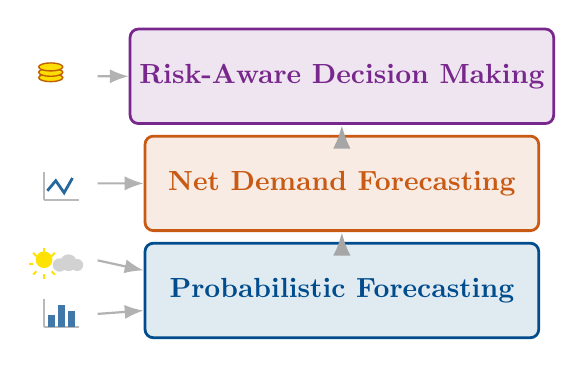
\begin{tikzpicture}[scale=0.85,
      layer/.style={rounded corners=3pt,minimum width=5cm,minimum height=1.2cm,
                    align=center,font=\bfseries,line width=1pt},
      feed/.style={-{Latex[length=2.4mm]},thick,gray!60},
      up/.style={-{Latex[length=3mm]},line width=1.3pt,gray!70}]

    % ---- Layer 1 (bottom): Probabilistic Forecasting ------------------
    \node[layer,draw=nogablue,fill=nogablue!12,text=nogablue] (l1) at (5.5,0.6)
          {Probabilistic Forecasting};
    \iconweather{(1.05,1.0)}
    \iconbars{(1.05,0.05)}
    \draw[feed] (1.85,1.05) -- ([yshift=3mm]l1.west);
    \draw[feed] (1.85,0.25) -- ([yshift=-3mm]l1.west);

    % ---- Layer 2 (middle): Net Demand Forecasting ----------------------
    \node[layer,draw=netorange,fill=netorange!12,text=netorange] (l2) at (5.5,2.2)
          {Net Demand Forecasting};
    \iconline{(1.05,1.95)}
    \draw[feed] (1.85,2.2) -- (l2.west);
    \draw[up] (l1.north) -- (l2.south);

    % ---- Layer 3 (top): Risk-Aware Decision Making ---------------------
    \node[layer,draw=riskpurple,fill=riskpurple!12,text=riskpurple] (l3) at (5.5,3.8)
          {Risk-Aware Decision Making};
    \iconcoins{(1.15,3.78)}
    \draw[feed] (1.85,3.8) -- (l3.west);
    \draw[up] (l2.north) -- (l3.south);
  \end{tikzpicture}
\end{frame}

% ============ Point Prediction vs. Probabilistic Forecasting ==========
\begin{frame}{Tomorrow's Demand?}
  \begin{columns}[T,onlytextwidth]

    % ---- Left: point prediction --------------------------------------
    \begin{column}{0.30\textwidth}
      \centering
      {\large\textbf{Point prediction}}\\[0.3em]
      \vfill
      {\usebeamercolor[fg]{structure}\fontsize{120}{120}\selectfont\textbf{7}}
      \vfill
    \end{column}

    \hfill\vrule\hfill

    % ---- Right: probabilistic forecast (3x3 grid) --------------------
    \begin{column}{0.66\textwidth}
      \centering
      {\large\textbf{Probabilistic forecast}}\\[0.4em]
      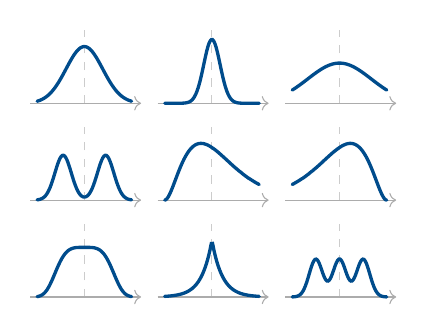
\begin{tikzpicture}[scale=0.60]
        % Pin the bounding box to the full 3x3 grid so revealing cells
        % one-by-one never re-centres the picture (no layout shift).
        \useasboundingbox (-0.2,-4.2) rectangle (7.65,1.6);
        % Row 0 -- revealed one by one
        \dcell{2-}{0}{0}{1.20*exp(-((\x-1)*(\x-1))/0.30)}                                  % normal
        \dcell{3-}{1}{0}{1.35*exp(-((\x-1)*(\x-1))/0.06)}                                  % small variance
        \dcell{4-}{2}{0}{0.85*exp(-((\x-1)*(\x-1))/0.90)}                                  % large variance
        % Rows 1 & 2 -- revealed together
        \dcell{5-}{0}{1}{0.95*exp(-((\x-0.55)*(\x-0.55))/0.06)+0.95*exp(-((\x-1.45)*(\x-1.45))/0.06)} % bimodal
        \dcell{5-}{1}{1}{15*(\x*\x)*exp(-2.6*\x)}                                          % right skew
        \dcell{5-}{2}{1}{15*((2-\x)*(2-\x))*exp(-2.6*(2-\x))}                              % left skew
        \dcell{5-}{0}{2}{1.05*exp(-((((\x-1)*(\x-1))/0.45)^2))}                            % plateau / uniform
        \dcell{5-}{1}{2}{1.20*exp(-abs(\x-1)/0.22)}                                        % heavy peak (Laplace)
        \dcell{5-}{2}{2}{0.80*exp(-((\x-0.5)*(\x-0.5))/0.04)+0.80*exp(-((\x-1)*(\x-1))/0.04)+0.80*exp(-((\x-1.5)*(\x-1.5))/0.04)} % trimodal
      \end{tikzpicture}\\[0.2em]
      \onslide<5->{\footnotesize all with mean $=7$}
    \end{column}

  \end{columns}
\end{frame}


% ===== Net Demand and Renewable Generation Forecasting ================
\begin{frame}{Net Demand $=$ Total Demand $-$ Renewable Generation}
  \centering
  \vspace{0.3em}
  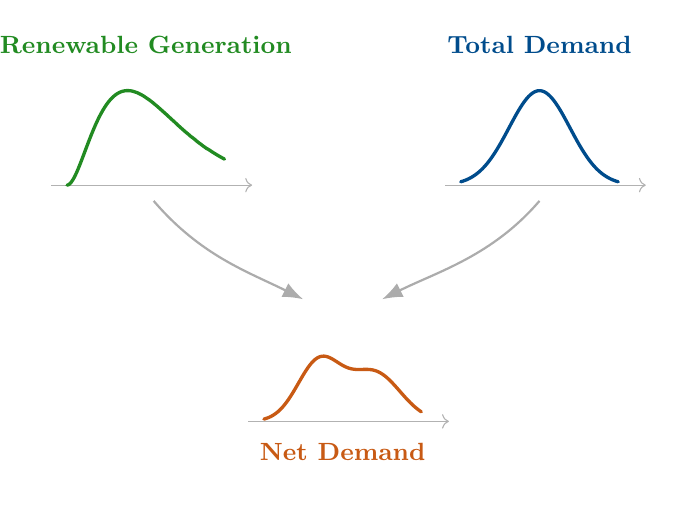
\begin{tikzpicture}[scale=1.0]
    % Pin the bounding box so revealing the panels/net curve does not
    % re-centre the picture (no layout shift across overlays).
    \useasboundingbox (-0.5,-0.7) rectangle (7.5,5.0);

    % ---- Top-left: renewable generation forecast (skewed, bounded) ---
    \panel{1}{(0,3)}{renewgreen}{Renewable Generation}{15*(\x*\x)*exp(-2.6*\x)}

    % ---- Top-right: total demand forecast (near-normal) --------------
    \panel{2}{(5,3)}{nogablue}{Total Demand}{1.20*exp(-((\x-1)*(\x-1))/0.30)}

    % ---- Converging arrows + combined net-demand distribution --------
    \only<3->{
      \draw[-{Latex[length=2.6mm]},thick,gray!65]
            (1.1,2.8) .. controls (1.7,2.1) and (2.3,1.9) .. (3.0,1.55);
      \draw[-{Latex[length=2.6mm]},thick,gray!65]
            (6.0,2.8) .. controls (5.4,2.1) and (4.7,1.9) .. (4.0,1.55);

      % bottom-centre: net demand -- wider, more volatile, irregular
      \begin{scope}[shift={(2.5,0)}]
        \draw[->,gray!60] (-0.2,0) -- (2.35,0);
        \draw[very thick,netorange,line cap=round]
              plot[domain=0:2,samples=90,smooth]
              (\x,{0.75*exp(-((\x-0.7)*(\x-0.7))/0.15)+0.62*exp(-((\x-1.4)*(\x-1.4))/0.22)});
        \node[netorange,anchor=north,font=\small\bfseries] at (1,-0.15) {Net Demand};
      \end{scope}
    }
  \end{tikzpicture}\\[0.4em]
  % The title states the identity for the *quantities*; this caveat states
  % that it does not carry over to their *distributions*.  The minipage
  % keeps the two sentences on two balanced lines instead of spilling.
  {\footnotesize\bfseries\color{netorange}
   \onslide<4->{%
     \begin{minipage}{0.88\textwidth}\centering
       Demand and renewable generation are strongly dependent.\\
       The marginals do not determine the difference --- model the joint law.
     \end{minipage}}}
\end{frame}

% ===================== Risk-Aware Prediction ==========================
\begin{frame}{Risk-Aware Prediction}
  \centering
  \vspace{0.1em}
  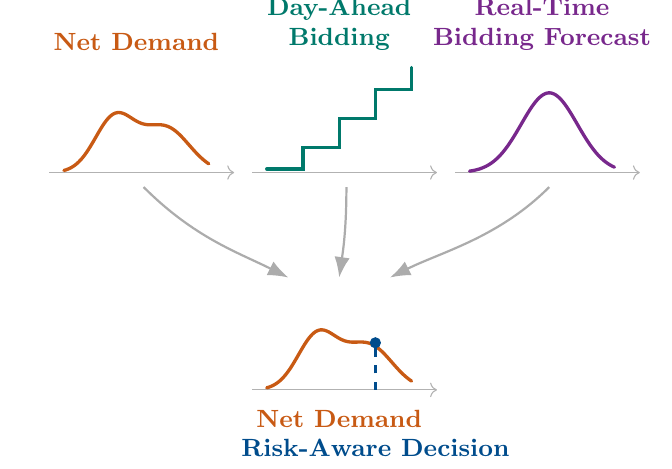
\begin{tikzpicture}[scale=0.92]
    % Pin the bounding box so revealing the panels/decision does not
    % re-centre the picture (no layout shift across overlays).
    \useasboundingbox (-0.5,-0.7) rectangle (8.0,5.0);

    % ---- Top-left: net demand forecast distribution -------------------
    \panel{1}{(0,3)}{netorange}{Net Demand}%
          {0.75*exp(-((\x-0.7)*(\x-0.7))/0.15)+0.62*exp(-((\x-1.4)*(\x-1.4))/0.22)}

    % ---- Top-centre: day-ahead market bidding (monotone step function) -
    \steppanel{2}{(2.8,3)}{bidteal}{Day-Ahead\\Bidding}

    % ---- Top-right: real-time market bidding forecast (distribution) ---
    \panel{3}{(5.6,3)}{riskpurple}{Real-Time\\Bidding Forecast}%
          {1.10*exp(-((\x-1.1)*(\x-1.1))/0.30)}

    % ---- Converging arrows + risk-aware cost-optimal decision ---------
    \only<4->{
      \draw[-{Latex[length=2.6mm]},thick,gray!65]
            (1.1,2.8) .. controls (1.8,2.1) and (2.4,1.9) .. (3.1,1.55);
      \draw[-{Latex[length=2.6mm]},thick,gray!65]
            (3.9,2.8) .. controls (3.9,2.2) and (3.85,1.9) .. (3.8,1.55);
      \draw[-{Latex[length=2.6mm]},thick,gray!65]
            (6.7,2.8) .. controls (6.0,2.1) and (5.2,1.9) .. (4.5,1.55);

      % bottom-centre: net demand distribution with the biased,
      % cost-optimal decision quantile marked
      \begin{scope}[shift={(2.8,0)}]
        \draw[->,gray!60] (-0.2,0) -- (2.35,0);
        \draw[very thick,netorange,line cap=round]
              plot[domain=0:2,samples=90,smooth]
              (\x,{0.75*exp(-((\x-0.7)*(\x-0.7))/0.15)+0.62*exp(-((\x-1.4)*(\x-1.4))/0.22)});
        \draw[nogablue,thick,dashed] (1.5,0) -- (1.5,0.65);
        \fill[nogablue] (1.5,0.65) circle (2.2pt);
        \node[netorange,anchor=north,font=\small\bfseries] at (1,-0.15) {Net Demand};
        \node[nogablue,anchor=north,font=\small\bfseries] at (1.5,-0.55) {Risk-Aware Decision};
      \end{scope}
    }
  \end{tikzpicture}
\end{frame}

% ========== Full Distribution vs. Confidence Interval =================
\begin{frame}{Full Distribution vs.\ Confidence Interval}
  \centering
  \vspace{0.2em}
  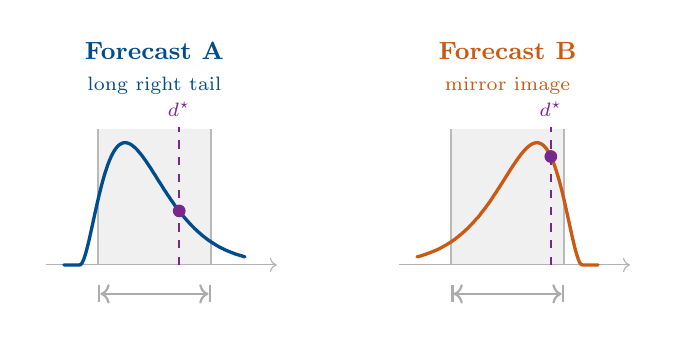
\begin{tikzpicture}[scale=1.15]
    % Pin the bounding box to both panels so revealing them one by one
    % never re-centres the picture (no layout shift).
    \useasboundingbox (-0.4,-0.75) rectangle (6.45,2.62);

    % Forecast A: gamma(k=3, rate 4) shifted to s=0.17624, peak scaled to 1.35
    \cipanel{1}{(0,0)}{nogablue}{Forecast A\\\scriptsize\mdseries long right tail}%
          {39.9009*((\x-0.17624)^2)*exp(-4*(\x-0.17624))*(\x>0.17624)}
    % Forecast B: exactly A reflected about x=1  (substitute \x -> 2-\x)
    \cipanel{2}{(3.9,0)}{netorange}{Forecast B\\\scriptsize\mdseries mirror image}%
          {39.9009*((1.82376-\x)^2)*exp(-4*(1.82376-\x))*(\x<1.82376)}

    % Cost-optimal reserve: the 5/6 quantile of each density (5:1 penalty).
    % Computed separately per curve -- see the note on \decision.
    \only<4->{
      \decision{(0,0)}{1.2736}{0.5962}
      \decision{(3.9,0)}{1.4777}{1.1971}
    }
  \end{tikzpicture}\\[0.2em]
  {\footnotesize\bfseries\color{nogablue}
   \onslide<3->{Identical 90\% interval --- mirrored tail risk}}

  \vspace{0.7em}
  \begin{itemize}[leftmargin=1.4em,itemsep=0.35em]
    \footnotesize
    \item<5-> Same endpoints, mirrored shape: the interval cannot tell a
              shortfall risk from a surplus risk.
    \item<6-> A cost-optimal decision integrates the density,
              $\int c(d,y)\,p(y)\,\mathrm{d}y$ --- two endpoints cannot supply it.
              Under a 5:1 under-prediction penalty the two forecasts call for
              visibly different reserves $d^\star$.
    \item<7-> One density serves every risk level: any quantile, any reserve
              margin, no refitting.
  \end{itemize}
\end{frame}

% ===================== Solution ========================================
\begin{frame}{Solution: Two Routes to a Full Distribution}
  \centering
  \vspace{0.2em}
  \begin{columns}[T,onlytextwidth]

    % ---- Left: Gaussian head -----------------------------------------
    \begin{column}{0.48\textwidth}
      \centering
      {\bfseries\color{nogablue} Deep network, Gaussian head}\\[0.15em]
      {\scriptsize the network outputs $(\mu,\sigma)$}\\[0.35em]
      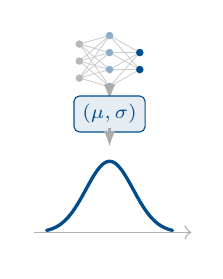
\begin{tikzpicture}[scale=0.8]
        \useasboundingbox (-0.3,-0.3) rectangle (2.35,3.25);
        \iconnet{(0.52,2.45)}{nogablue}
        \draw[-{Latex[length=2mm]},thick,gray!65] (1.0,2.28) -- (1.0,2.10);
        \node[draw=nogablue,fill=nogablue!10,text=nogablue,rounded corners=2pt,
              inner sep=3pt,font=\scriptsize] at (1.0,1.88) {$(\mu,\sigma)$};
        \draw[-{Latex[length=2mm]},thick,gray!65] (1.0,1.66) -- (1.0,1.36);
        \draw[->,gray!60] (-0.2,0) -- (2.30,0);
        % amplitude set so both panels enclose the same area (1.05)
        \draw[very thick,nogablue,line cap=round]
              plot[domain=0:2,samples=90,smooth] (\x,{1.1280*exp(-((\x-1)*(\x-1))/0.28)});
      \end{tikzpicture}\\[0.35em]
      {\scriptsize closed form, cheap, calibrated spread\\
       \color{gray!45!black} but always unimodal and symmetric}
    \end{column}

    % ---- Right: normalizing flow --------------------------------------
    \begin{column}{0.48\textwidth}
      \centering
      \onslide<2->{%
      {\bfseries\color{riskpurple} Normalizing flow}\\[0.15em]
      {\scriptsize the network conditions an invertible map $f_\theta$}\\[0.35em]
      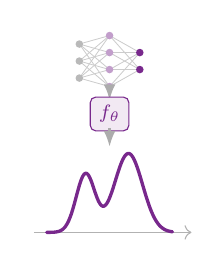
\begin{tikzpicture}[scale=0.8]
        \useasboundingbox (-0.3,-0.3) rectangle (2.35,3.25);
        \iconnet{(0.52,2.45)}{riskpurple}
        \draw[-{Latex[length=2mm]},thick,gray!65] (1.0,2.28) -- (1.0,2.10);
        \node[draw=riskpurple,fill=riskpurple!10,text=riskpurple,rounded corners=2pt,
              inner sep=3pt,font=\scriptsize] at (1.0,1.88) {$f_\theta$};
        \draw[-{Latex[length=2mm]},thick,gray!65] (1.0,1.66) -- (1.0,1.36);
        \draw[->,gray!60] (-0.2,0) -- (2.30,0);
        % Deliberately skewed *and* bimodal: a shape no Gaussian head can reach.
        % Amplitudes scaled so this encloses the same area as the Gaussian (1.05).
        \draw[very thick,riskpurple,line cap=round]
              plot[domain=0:2,samples=120,smooth]
              (\x,{0.9262*exp(-((\x-0.62)*(\x-0.62))/0.045)
                  +1.2531*exp(-((\x-1.30)*(\x-1.30))/0.10)});
      \end{tikzpicture}\\[0.35em]
      {\scriptsize exact likelihood, $p(y)=\varphi(f_\theta(y))\,|f_\theta'(y)|$\\
       \color{gray!45!black} any shape: skew, multimodality, heavy tails}}
    \end{column}

  \end{columns}

  \vspace{0.7em}
  {\footnotesize\bfseries\color{netorange}
   \onslide<3->{A Gaussian head cannot represent Forecast A or B --- the flow can.}}\\[0.3em]
  {\footnotesize\color{nogablue}
   \onslide<4->{Both fit by maximum likelihood; ranked by proper scores
   \emph{and} by operational cost.}}
\end{frame}

% ===================== Recap ===========================================
\begin{frame}{Recap}
  \centering
  \begin{tikzpicture}[scale=0.95,
      layer/.style={rounded corners=3pt,minimum width=5cm,minimum height=1.2cm,
                    align=center,font=\bfseries,line width=1pt},
      feed/.style={-{Latex[length=2.4mm]},thick,gray!60},
      up/.style={-{Latex[length=3mm]},line width=1.3pt,gray!70}]
    % Pin the bounding box to the full 3-layer stack so building it up
    % bottom-to-top does not re-centre the picture (no layout shift).
    \useasboundingbox (0.6,-0.25) rectangle (8.2,4.55);

    % ---- Layer 1 (bottom): Probabilistic Forecasting ----------------
    \only<1->{
      \node[layer,draw=nogablue,fill=nogablue!12,text=nogablue] (l1) at (5.5,0.6)
            {Probabilistic Forecasting};
      \iconweather{(1.05,1.0)}
      \iconbars{(1.05,0.05)}
      \draw[feed] (1.85,1.05) -- ([yshift=3mm]l1.west);
      \draw[feed] (1.85,0.25) -- ([yshift=-3mm]l1.west);
    }

    % ---- Layer 2 (middle): Net Demand Forecasting -------------------
    \only<2->{
      \node[layer,draw=netorange,fill=netorange!12,text=netorange] (l2) at (5.5,2.2)
            {Net Demand Forecasting};
      \iconline{(1.05,1.95)}
      \draw[feed] (1.85,2.2) -- (l2.west);
      \draw[up] (l1.north) -- (l2.south);
    }

    % ---- Layer 3 (top): Risk-Aware Decision Making ------------------
    \only<3->{
      \node[layer,draw=riskpurple,fill=riskpurple!12,text=riskpurple] (l3) at (5.5,3.8)
            {Risk-Aware Decision Making};
      \iconcoins{(1.15,3.78)}
      \draw[feed] (1.85,3.8) -- (l3.west);
      \draw[up] (l2.north) -- (l3.south);
    }
  \end{tikzpicture}
\end{frame}

% ===================== Preliminary Results ============================
\begin{frame}{Preliminary Results}
  \centering
  \vfill
  {\large\bfseries\usebeamercolor[fg]{structure}Operational Cost Reduction}\\[1.2em]
  \begin{columns}[c,onlytextwidth]
    \begin{column}{0.46\textwidth}
      \centering
      \resizebox{!}{0.85cm}{\color{nogablue}\textbf{40\%\,--\,73\%}}
    \end{column}
    \begin{column}{0.08\textwidth}
      \centering\rule{0.6pt}{2.2cm}
    \end{column}
    \begin{column}{0.46\textwidth}
      \centering
      \resizebox{!}{0.85cm}{\color{netorange}\textbf{8\%\,--\,17\%}}
    \end{column}
  \end{columns}
  \vfill
\end{frame}

% ===================== Operational Value ===============================
\begin{frame}{Operational Value, Innovation \& Alignment}
  \centering
  \begin{columns}[T,onlytextwidth]

    % ---- Operational value ---------------------------------------------
    \begin{column}{0.33\textwidth}
      \centering
      {\bfseries\color{nogablue} Operational Value}\\[0.6em]
      \begin{itemize}[leftmargin=1.2em,itemsep=0.5em]
        \footnotesize
        \item 40--73\% cost reduction, extended from point forecasts to full distributions
        % \item Reserve-sizing tool with finite-sample coverage guarantees
        \item Net-demand capability for a high-renewables grid
        \item Deployable prototype \& knowledge transfer to NOGA
      \end{itemize}
    \end{column}

    % ---- Innovation ------------------------------------------------------
    \begin{column}{0.33\textwidth}
      \centering
      {\bfseries\color{riskpurple} Innovation}\\[0.6em]
      \begin{itemize}[leftmargin=1.2em,itemsep=0.5em]
        \footnotesize
        \item First \emph{calibrated, integrated} demand \& renewable distributions under a cost objective
        \item Techniques compared by proper scores \emph{and} operational cost
        \item Characterises when joint vs.\ marginal dependence modelling pays off
        \item De-risked: builds on a validated 3-year data pipeline
      \end{itemize}
    \end{column}

    % ---- Alignment with the call ------------------------------------------
    \begin{column}{0.33\textwidth}
      \centering
      {\bfseries\color{netorange} Alignment with the Call}\\[0.6em]
      \begin{itemize}[leftmargin=1.2em,itemsep=0.5em]
        \footnotesize
        \item Primary domain \textbf{2.5} --- demand forecasting
        \item \S2.1.5 reserve \& stability
        \item \S2.2.2 monitoring \& state forecasting
        \item \S2.1.6 renewable integration
        \item \S2.4.3 operation under limited reserves
      \end{itemize}
    \end{column}

  \end{columns}
\end{frame}

% ===================== Work Plan =======================================
\begin{frame}{Work Plan}
  \centering
  \resizebox{\textwidth}{!}{%
  \begin{ganttchart}[
      hgrid, vgrid,
      x unit=0.92cm,
      y unit chart=0.7cm,
      y unit title=0.6cm,
      bar/.append style={fill=nogablue!65},
      bar height=0.6,
      group/.append style={fill=nogablue},
      group right shift=0, group left shift=0, group peaks height=0,
      milestone/.append style={fill=nogablue!50!red},
      progress label text={}, link/.style={->},
      title/.append style={fill=nogablue!15},
      bar label font=\normalsize, group label font=\bfseries\normalsize,
      title label font=\bfseries\normalsize, milestone label font=\normalsize,
      ]{1}{12}
      \gantttitle{Project month}{12} \\
      \gantttitlelist{1,...,12}{1} \\
      \ganttgroup{WP1 --- Data \& Benchmark (T1)}{1}{4} \\
      \ganttgroup{WP2 --- Demand Forecasting (T2)}{3}{7} \\
      \ganttgroup{WP3 --- Renewable Forecasting (T3)}{4}{8} \\
      \ganttgroup{WP4 --- Net-Demand Integration (T4)}{7}{10} \\
      \ganttgroup{WP5 --- Decision Layer \& Validation (T5)}{9}{12} \\
      \ganttgroup{WP6 --- Management \& Dissemination}{1}{12} \\
      \ganttmilestone{}{1}\ganttmilestone{}{4}\ganttmilestone{}{7}%
      \ganttmilestone{}{10}\ganttmilestone{}{12}
  \end{ganttchart}%
  }\\[1em]
  {\footnotesize\bfseries\color{nogablue} 12-month project, six work packages}\\[0.6em]
  {\footnotesize \textbf{M1} kick-off \quad \textbf{M4} benchmark released \quad
   \textbf{M7} calibrated demand \& renewable models \quad
   \textbf{M10} integrated net-demand distribution \quad
   \textbf{M12} deployable prototype}
\end{frame}

% ===================== Budget ==========================================
\begin{frame}{Budget}
  \centering
  \vspace{0.2em}
  {\footnotesize
  \begin{tabular}{@{}llrrr@{}}
    \toprule
    \textbf{Person} & \textbf{Role} & \textbf{\% Pos.} & \textbf{Months} & \textbf{Budget (NIS)} \\
    \midrule
    Or Aleksandrowicz        & Principal Researcher 1          & 20\% & 12 & --- (in kind) \\
    Avigdor Gal              & Principal Researcher 2          & 5\%  & 12 & --- (in kind) \\
    Gilad Kutiel             & Co-Researcher / Project Manager & 66\% & 12 & 182{,}160 \\
    Research assistant (TBD) & Data processing                 & 20\% & 12 & 35{,}040 \\
    \bottomrule
  \end{tabular}}

  \vspace{1.4em}
  \begin{columns}[c,onlytextwidth]
    \begin{column}{0.5\textwidth}
      \centering
      {\footnotesize
      \begin{tabular}{@{}lr@{}}
        \toprule
        \textbf{Item} & \textbf{Amount (NIS)} \\
        \midrule
        Personnel               & 217{,}200 \\
        AI \& cloud processing  & 10{,}000 \\
        Overhead (15\%)         & 34{,}080 \\
        \midrule
        \textbf{Total}          & \textbf{261{,}280} \\
        \bottomrule
      \end{tabular}}
    \end{column}
    \begin{column}{0.42\textwidth}
      \centering
      \resizebox{0.95\linewidth}{!}{\color{nogablue}\textbf{NIS 261{,}280}}\\[0.3em]
      {\scriptsize 12-month total \textbullet\ overhead 15\% \textbullet\ PIs in kind}
    \end{column}
  \end{columns}
\end{frame}

% ===================== Questions and Discussion =======================
\begin{frame}{Questions and Discussion}
  \centering
  \vfill
  {\usebeamercolor[fg]{structure}\fontsize{200}{200}\selectfont\textbf{?}}
  \vfill
\end{frame}

\end{document}
